\begin{chapter}{Introduction}
\label{ch:introduction}
Various forms of noise occur in many forms of data acquisition, transmission and processing.
This noise needs to be removed in order to obtain a meaningful interpretation of the data, to enable further processing or, as in many image processing 
applications, just for aesthetic reasons. A common everyday example for a noisy image is taking a picture with a digital camera (e.g. integrated in a smart phone) in a weakly illuminated room:
Especially the dark areas of the picture are not uniform in color and brightness, but have small variations from pixel to pixel.\\

A noise removal algorithm needs to remove these small variations, but at the same time not alter important features of the data. In the case of images important features are for example 
the edges separating areas of different colors and providing the necessary sharpness of the picture. These edges, on the other hand, are characterized by large variations. The distinction
between small and large variations is also helpful in the task of inpainting, which tries to restore the picture at unknown or damaged regions.\\

The method of total variation(TV) noise removal, which has the above described capabilities, was first introduced by Rudin, Osher and Fatemi \cite{RudinOsher} in 1992
for the case of real-valued, that means grayscale images. Their method is briefly summarized in the following section.

\section{Grayscale images}
Let $u_0:  \mathbb{R}\supset\Omega\to \mathbb{R}$ describe the original, noise-free image where the image domain $\Omega$ is usually a rectangular or cuboid subset of $\mathbb{R}^2$ or $\mathbb{R}^3$, respectively. 
Assuming the original picture is corrupted by Gaussian noise $n: \Omega\to\mathbb{R}$ with zero mean and variance $\sigma^2$, the noisy picture is given by $u: \Omega\to \mathbb{R}$ where
$u = u_0 + n$. The edge-preserving denoising of the picture is then equivalent to the solution $u^* :\Omega\to \mathbb{R}$ of the following constrained optimization problem:
\begin{align}
    \label{osher_opt}
    u^* &= \operatorname{argmin}_{f: \Omega\to \mathbb{R}}\int_\Omega\left\vert\nabla u\right\vert \mathop{dx} \quad\text{s.t.}\\
    \int_\Omega(u-u_0)\mathop{dx} &= 0, \quad\text{and} \int_\Omega(u-u_0)^2 \mathop{dx}= \sigma^2
\end{align}

The first term, $TV(u)=\int_\Omega\left\vert\nabla u\right\vert\mathop{dx}$, is called the total variation of $u$. Rudin, Osher and Fatemi then use a partial differential equation (PDE) approach to solve
the corresponding Euler-Lagrange equation for (\ref{osher_opt}). Later, Chambolle and Lions \cite{ChambolleLions} showed that (\ref{osher_opt}) is equivalent to the minimization of
the functional
\begin{equation}
    \label{osher_func}
    J(u)=\frac{1}{2}\norm{u-u_0}_2^2 +\lambda \int_\Omega\left\vert\nabla u\right\vert\mathop{dx}.
\end{equation}

\subsection{Edge preservation} % (fold)
\label{sub:Edge preservation}
A basic intuition why the $L^1$ norm in (\ref{osher_func}) is better suited for conserving sharp discontinuities, such as edges, can be seen from the following plot, taken from \cite{SceneFlow}. The gradients in the integral expressions are to be understood in terms of their finite differences approximations with $\nabla f=f(x_{i+1})-f(x_i)/h$ with some $h=1/M<1/N$, $x_i=0$ and $x_{i+1}=x_i+h$.\\
 
\begin{figure}[h!]
        \centering
	    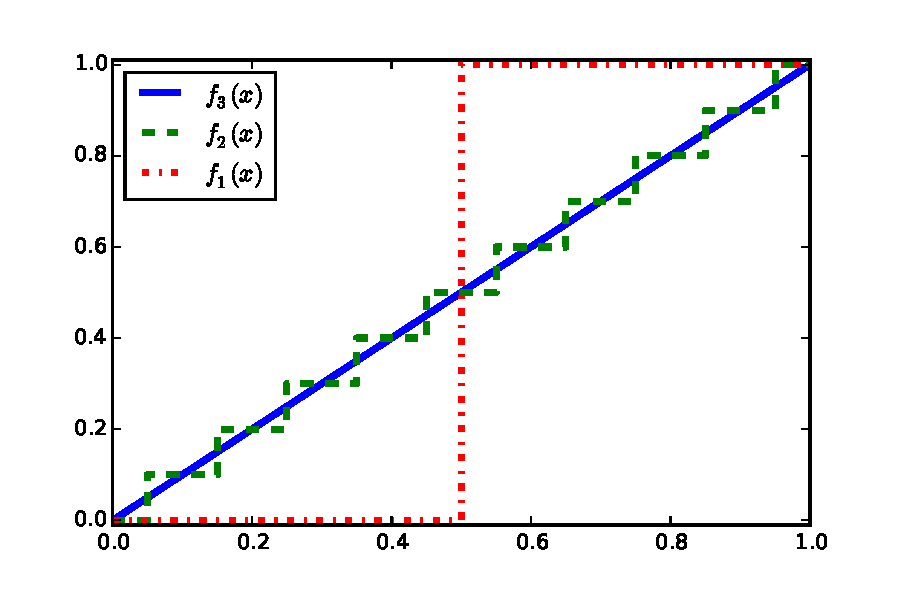
\includegraphics[width=0.9\linewidth]{./figures/introduction/tv12comparison.pdf}
	\caption[Comparison total variation]{Plots of three functions with ($N=1,\;10,\;100$) steps and a total variation equal to $1.0$}
	\label{fig:tv12comparison}
\end{figure}
\begin{table}[h!]
\centering
\begin{tabular}{|l|l|l|}
    \hline
    \textbf{Function} & $\int_{[0,1]}\left\vert\nabla f\right\vert\mathop{dx}$ & $\int_{[0,1]}\left\vert\nabla f\right\vert^2\mathop{dx}$ \\
    \hline
    $f_1$ & 1.0 & 1.0 \\
    $f_2$ & 1.0 & 0.1 \\
    $f_3$ & 1.0 & 0.01 \\
    \hline
\end{tabular}
\end{table}

One can see that the $L^2$ variation term favours continuous transitions, such as $f_3$, rather than the sudden jump in $f_1$ whereas the total variation is the same for
all cases.
% subsection Edge preservation (end)


\subsection{Discretization} % (fold)
\label{sub:Discretization}
For a grayscale image $u:\Omega\subset\mathbb{R}^2\to\mathbb{R}$ a discrete grid of pixels 
$\Omega=\lbrace 1,2,\ldots,m\rbrace\times\lbrace1,2,\ldots,n\rbrace\subset\mathbb{R}^2$ is chosen. The picture $u$ then takes the values $u_{i,j}:=u((i,j))\in [0,1]$
at the points $(i,j)\in\Omega$, and a forward finite difference discretization of the gradient $\nabla u:=(u_x,u_y)^T$ can be used, where
\begin{align}
    (u_x)_{i,j} &= 
	\begin{cases}
	u_{i,j+1}-u_{i,j}, & 1\leq j < n \\
	0, & j=n 
	\end{cases} \\
    (u_y)_{i,j} &= 
	\begin{cases}
	u_{i+1,j}-u_{i,j}, & 1\leq i < m \\
	0, &i=m
	\end{cases}.\nonumber
\end{align}

This leads to the \emph{isotropic} TV functional
\begin{equation}
    \label{eq:original_isofunctional}
    TV_{iso}(u)=\sum_{i,j}\sqrt{(u_{i+1,j}-u_{i,j})^{2}+(u_{i,j+1}-u_{i,j})^{2}}.
\end{equation}

This TV term corresponds to the formulation originally proposed by Rudin et al\cite{RudinOsher}, where $\left\vert\nabla u\right\vert=\sqrt{u_x^{2}+u_y^{2} }$.
Another possibility is the \emph{anisotropic} version of the functional, which allows for more flexibility in the reweighting process, described in \ref{sub:IRLS}, and is even necessary for the proximal point algorithm, described in \ref{sub:ProximalPoint}.
It is given by
\begin{equation}
    \label{eq:original_anisofunctional}
    TV_{aniso}(u)=\sum_{i,j}|u_{i+1,j}-u_{i,j}|+|u_{i,j_1}-u_{i,j}|.
\end{equation}

For the total functional, the pixel-wise differences to the original picture $u_0$ need to be added
\begin{equation}
    \label{eq:original_functional}
    J(u)=\sum_{i,j}(u_{i,j}-(u_0)_{i,j})^2 + \lambda TV(u).
\end{equation}


% subsection Discretization(end)


\section{Color Images}
The next step in the development of image denoising algorithms was their generalization to color images. From a mathematical perspective this just means considering pictures
from $\Omega\to C\simeq \mathbb{R}^3$ where the form and additional properties of $C$ depend on the chosen color model. \\
In the most simple case of linear models, like RGB for instance, one could choose $C$ as $[0,1]^3$ and consider denoising each component individually (channel-by-channel model)
or consider $\mathbb{R}^3$ as a normed vector space of tuples $(x_R, x_G, x_B)$ (linear-vectorial model).\\
For the nonlinear models, especially the so-called chromaticity-brightness model, investigated by Chang and March \cite{Kang}, shows the closest resemblance to human perception.
In this case, take $C=S^2\times [0,1]$ such that the chromaticitiy takes values on the sphere $S^2$ considered as a submanifold of the Euclidean space $\mathbb{R}^3$, 
while the brightness is real-valued, as in the case of grayscale images.

\section{Manifold-valued Images} % (fold)
\label{sec:Manifold-valued Images}
Just by changing the color model from a linear to a non-linear one, pixels become non-trivially manifold-valued.
Apart from non-linear color models, more complicated data arises in a variety of applications such as Diffusion Tensor Magnetic Resonance Imaging (DTI-MRI), computer vision and robotics to name just a few. In most cases this data can
be represented by matrices such that the pixels become matrix-valued as well. In addition to that, the model underlying
the data and the process of data acquisition result in a set of constraints imposed on the matrices. The set of matrices
defined by those constraints often allows for a differentiable structure thus enabling geometric optimization methods.
For most types of manifold-data also "edges" in the data, for example between two neighboring, homogeneous areas of 
different orientations in the case of $SO(3)$ data, are considered a feature that needs to be preserved.
Since also manifold-valued data is subject to noise, the generalization of the algorithm to manifold valued data is the
next logical step.


\section{Objective and Outline of this thesis}
In this thesis the Manifold Total Variation Minimization Template Library (MTVMTL), an extendable multi-threaded C++ template library for the purpose of TV minimization of manifold-valued images is introduced. 
The implemented minimization algorithms are based on the iteratively reweighted least squares (IRLS) adaption suggested by Sprecher and Grohs \cite{SprecherIRLS} as well as a 
proximal point algorithm by Weinmann et al \cite{Weinmann}. The implementation is extended to 3D image cubes, the Grassmann manifold and also some quasi-analytic expressions for derivatives of the Riemannian distance function are provided.\\

In the following Chapter 2 a short summary of the necessary theory, a description of the algorithms and relevant properties for each of the implemented manifolds is provided.
After that, Chapter 3 introduces the library itself and in particular its capabilities, design concepts, structure, installation and usage in the form of some typical
use cases. In Chapter 4 numerical experiments are conducted, showing various application of the library as well as convergence behavior and comparisons between 
IRLS and proximal point based algorithms.\\

Finally, chapter 5 concludes with possible extensions and adaptions of the library, in particular possibility of recursive splitting of the image domain into smaller subproblems and
the transition to distributed architectures.
% section Manifold-valued Images (end)
\end{chapter}
